With the representation of the symbol of high-order PDE operators given in Definition \ref{def:high_order_symbol}, we can derive the symbol of multigrid error propagation operators.

The total multigrid error propagation operator is given by
\begin{equation}
\mathbf{E}_{\text{TMG}} = {\color{burgundy}\mathbf{S}}_f \left( \mathbf{I} - {\color{burgundy}\mathbf{P}}_{\text{ctof}} {\color{burgundy}\mathbf{A}}_c^{-1} {\color{burgundy}\mathbf{R}}_{\text{ftoc}} {\color{burgundy}\mathbf{A}}_f \right) {\color{burgundy}\mathbf{S}}_f
\end{equation}
where ${\color{burgundy}\mathbf{S}}_f$ represents the smoother error propagation operator, while ${\color{burgundy}\mathbf{P}}_{\text{ctof}}$ and ${\color{burgundy}\mathbf{R}}_{\text{ftoc}}$ represent the grid prolongation and restriction operators between the coarse and fine grids, respectively.

\begin{definition}
The symbol of total multigrid error propegation operator for a finite element operator ${\color{burgundy}\mathbf{A}}$ is given by
\begin{equation}
\tilde{\mathbf{E}}_{\text{TMG}} \left( \mathbf{\theta} \right) = \tilde{{\color{burgundy}\mathbf{S}}}_f \left( \mathbf{\theta}, \omega \right) \left( \mathbf{I} - \tilde{{\color{burgundy}\mathbf{P}}}_{\text{ctof}} \left( \mathbf{\theta} \right) \left(\tilde{{\color{burgundy}\mathbf{A}}}_c \left( \mathbf{\theta} \right) \right)^{-1} \tilde{{\color{burgundy}\mathbf{R}}}_{\text{ftoc}} \left( \mathbf{\theta} \right) \tilde{{\color{burgundy}\mathbf{A}}}_f \left( \mathbf{\theta} \right) \right) \tilde{{\color{burgundy}\mathbf{S}}}_f \left( \mathbf{\theta}, \omega \right)
\end{equation}
where $\tilde{{\color{burgundy}\mathbf{S}}}_f$ represents the smoother error propagation symbol with any additional parameters $\omega$, while $\tilde{{\color{burgundy}\mathbf{P}}}_{\text{ctof}}$ and $\tilde{{\color{burgundy}\mathbf{R}}}_{\text{ftoc}}$ represent the grid prolongation and restriction symbols, respectively.
\label{def:multigrid_symbol}
\end{definition}

This error propagation operator can represent both h-multigrid and p-multigrid, depending upon the grid transfer operators and coarse grid representation chosen.

% -- P-Multigrid --------------------------------------------------------------
\subsection{P-Multigrid}

In p-multigrid, the different grids have the same number and size of finite elements but with different order basis functions.
The grid transfer operators can be represented elementwise and can thus be easily represented in the form of Equation \ref{eq:libceed_representation}.

The prolongation operator from the coarse to the fine grid interpolates low-order basis functions at the nodes for the high-order basis functions.
Figure \ref{fig:pProlongation} shows the evaluation of second order basis function on the Gauss-Lobatto nodes for a fourth order basis.

\begin{figure}[!ht]
  \centering
  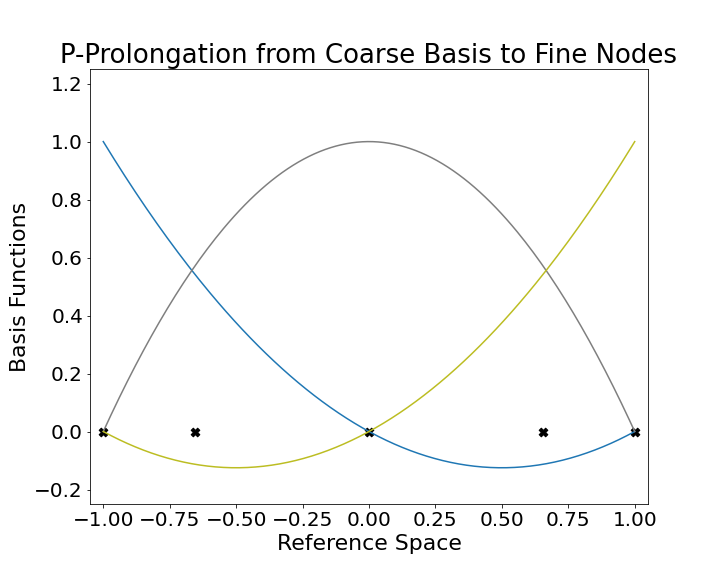
\includegraphics[width=0.48\textwidth]{../img/pProlongation}
  \caption{P-Prolongation from Coarse Basis to Fine Basis Points}
  \label{fig:pProlongation}
\end{figure}

The prolongation operator can be therefore be represented by
\begin{equation}
\begin{tabular}{c}
${\color{burgundy}\mathbf{P}}_{\text{ctof}} = \mathbf{P}_f^T \mathbf{G}_f^T {\color{burgundy}\mathbf{P}}_e \mathbf{G}_c \mathbf{P}_c$\\
${\color{burgundy}\mathbf{P}}_e = {\color{blue(ncs)}\mathbf{I}} {\color{applegreen}\mathbf{D}}_{\text{scale}} {\color{blue(ncs)}\mathbf{B}}_{\text{ctof}}$
\end{tabular}
\end{equation}
where ${\color{blue(ncs)}\mathbf{B}}_{ctof}$ is an interpolation operator from the coarse grid basis to the fine grid basis, $\mathbf{P}_f$ and $\mathbf{G}_f$ are the fine grid element assembly operators, $\mathbf{P}_c$ and $\mathbf{G}_c$ are the coarse grid element assembly operators, and ${\color{applegreen}\mathbf{D}}_{\text{scale}}$ is a scaling operator to account for node multiplicity across element interfaces.
Restriction from the fine grid to the coarse grid is given by the transpose, ${\color{burgundy}\mathbf{R}}_{\text{ftoc}} = {\color{burgundy}\mathbf{P}}_{\text{ctof}}^T$.

TODO: INSERT CHART SHOWING P-MULTIGRID PROLONGATION OPERATION

Following the derivation from Section \ref{sec:lfahighorder}, we can derive the symbols of ${\color{burgundy}\mathbf{P}}_{\text{ctof}}$ and ${\color{burgundy}\mathbf{R}}_{\text{ftoc}}$.

\begin{definition}
The symbol of the p-prolongation operator is given by
\begin{equation}
\tilde{{\color{burgundy}\mathbf{P}}}_{\text{ctof}} \left( \theta \right) = \mathbf{Q}_f^T \left( {\color{burgundy}\mathbf{P}}_e \odot \left[ e^{\imath \sum_d \left( \mathbf{x}_{i, f} - \mathbf{x}_{j, c} \right) \mathbf{\theta} / \mathbf{h}} \right] \right) \mathbf{Q}_c
\end{equation}
where $i \in \left[ 0, 1, \dots, p_{\text{fine}} \right]$, $h$ is the length of the element, and $j \in \left[ 0, 1, \dots, p_{\text{coarse}} \right]$.
The matrices $\mathbf{Q}_f$ and $\mathbf{Q}_c$ are the localization mappings for the fine and coarse grid, respectively, and the element p-prolongation operator is given by ${\color{burgundy}\mathbf{P}}_e = {\color{blue(ncs)}\mathbf{I}} {\color{applegreen}\mathbf{D}}_{\text{scale}} {\color{blue(ncs)}\mathbf{B}}_{\text{ctof}}$.
\label{def:p_prolongation_symbol}
\end{definition}

\begin{definition}
The symbol of p-restriction operator is given by the expression
\begin{equation}
\tilde{{\color{burgundy}\mathbf{R}}}_{\text{ftoc}} \left( \theta \right) = \mathbf{Q}_c^T \left( {\color{burgundy}\mathbf{R}}_e \odot \left[ e^{\imath \sum_d \left( \mathbf{x}_{i, c} - \mathbf{x}_{j, f} \right) \mathbf{\theta} / \mathbf{h}} \right] \right) \mathbf{Q}_f
\end{equation}
where $i \in \left[ 0, 1, \dots, p_{\text{coarse}} \right]$, $h$ is the length of the element, and $j \in \left[ 0, 1, \dots, p_{\text{fine}} \right]$.
The matrices $\mathbf{Q}_f$ and $\mathbf{Q}_c$ are the localization mappings for the fine and coarse grid, respectively, and the element p-restriction operator is given by ${\color{burgundy}\mathbf{R}}_e = {\color{burgundy}\mathbf{P}}_e^T = {\color{blue(ncs)}\mathbf{B}}_{\text{ctof}}^T {\color{applegreen}\mathbf{D}}_{\text{scale}} {\color{blue(ncs)}\mathbf{I}}$.
\label{def:p_restriction_symbol}
\end{definition}

% -- H-Multigrid --------------------------------------------------------------
\subsection{H-Multigrid}

TODO: H MULTIGRID
